\chapter{基于双通道注意力的极化信息提取方法}
\section{引言}
在上一章中,介绍了目标的散射信息可通过极化散射矩阵$S$进行表示,并通过对$S$进行矢量化分解,可以得到极化信息的进一步表征,包括极化相干矩阵$T$和极化协方差矩阵$C$。使用不同的散射基对$T$或$S$进行分解,得到具有不同物理含义的散射分量。在当前的极化SAR目标分类任务中,基于卷积神经网络(CNN)的分类器通常直接采用协方差矩阵和相干矩阵作为输入,而忽略了极化目标分解的特征表示方式\citing{}。在使用CNN进行分类时,由于其分层特征提取特性,前端网络提取的特征层次相对较低,可能未能充分提取极化SAR数据中的有用信息。同时,如果直接堆叠使用所有极化特征作为输入可能导致特征维度的大幅增加,并且多维特征之间必然存在着信息冗余,可能降低分类准确性\citing{}。

% 针对上述问题,本章研究了一种基于双通道注意力机制的极化信息提取方法。该方法以注意力机制为基础,设计双通道的联合注意力结构,联合不同层次的极化特征进行建模,通过两个单独注意力通道提取不同层次的极化特征并相互校正,最终得到可鉴别极化特征。

针对上述问题,本章提出了一种基于注意力机制的极化信息提取方法。鉴于不同的散射目标之间的散射特性存在差异,引入了关联注意力机制,联合不同层次的极化特征的关系进行联合建模。首先,为了提取不同层次的极化信息,设计了双通道注意力的极化信息提取网络结构,分别对应目标分解通道和散射数据通道。然后,在两个通道中分别利用空间、通道注意力机制,捕捉各自的关键信息。为了挖掘不同层次极化信息的联系,设计了权重融合模块,用于相互引导修正两个通道的注意力权重。最后,结合跨空间学习模块,对不同尺度的极化特征进行再次融合,得到有效的极化特征表示,结合后续的卷积网络与分类器完成目标分类任务。本章提出的双通道注意力的极化信息提取方法,可以作为一个即插即用的插件式组件,应用到现有的任意一个极化SAR目标分类网络中,增强极化信息的表征能力,提高最终的分类准确率。

\section{注意力机制介绍}
注意力机制是机器学习和深度学习中一种关键的技术,其主要目标是在处理信息是实现对输入数据的加权关注,以便网络模型能够更有效地捕捉与任务相关的信息。基于注意力机制的信息提取在自然语言处理、计算机视觉等领域获得了广泛的应用\citing{}。注意力机制使用不同的权重来表示输入特征的不同的重要程度,根据关注的角度差异,可以分为通道注意力、空间注意力和混合注意力三种类型。
\subsection{通道注意力机制}
输入深度网络的特征一般使用多维数据表示,通道注意力专注于挖掘不同通道间的关键,通过自适应地调整通道之间的权重,使网络模型能够更加聚焦于对后续任务有益的特征通道,从而提升模型的性能和泛化能力。压缩和激励网络(Squeeze-and-Extraction Networks, SENet)\citing{hu2018squeeze}是最具代表性的通道注意力实现模型。图\ref{SENet}为SENet的组成结构图,该方法由压缩和激励两个阶段构成。在压缩阶段,通过全局池化操作对输入多维特征进行压缩,将每个通道的信息整合成单一的数值,用于全局感受野的建模。对于维数是$H\times W \times C$的输入特征,压缩操作将其压缩为$1 \times 1 \times C$维,具体如下式所示:
\begin{equation}
    z_c=\mathbf{F}_{sq}\left( \mathbf{u}_c \right) =\frac{1}{H\times W}\sum_{i=1}^H{\sum_{j=1}^W{u\left( i,j \right)}}
\end{equation}

在激励阶段,利用全连接层和激活函数,学习得到每个通道的权重。得到的权重向量用来对原始输入特征图中的每个通道进行加权,形成加权的特征图。具体如下式所示:
\begin{equation}
    \mathbf{s}=\mathbf{F}_{ex}\left( \mathbf{z},\mathbf{W} \right) =\sigma \left( g\left( \mathbf{z},\mathbf{W} \right) \right) =\sigma \left( \mathbf{W}_2\sigma *\left( \mathbf{W}_1\mathbf{z} \right) \right)
\end{equation}
其中,$\sigma$表示ReLu激活函数\citing{nair2010rectified},$W_1 \in \mathbb{R}^{\frac{C}{r}\times C}$且$W_2 \in \mathbb{R}^{C \times \frac{C}{r}}$。

模型最终通过权重向量$s$来对输入进行重标定得到:
\begin{equation}
    \widetilde{\mathbf{x}}_c=F_{scale}\left( \mathbf{u}_c,s_c \right) =s_c\mathbf{u}_c
\end{equation}
其中,$ \widetilde{\mathbf{X}}=\left[ \widetilde{\mathbf{x}_1},\widetilde{\mathbf{x}_2},\cdots ,\widetilde{\mathbf{x}_C} \right] $, $F_{scale}\left( \mathbf{u}_c,s_c \right)$ 表示 $s_c$与特征图$\mathbf{u}_c \in \mathbb{R}^{H\times W}$的通道级乘积。


\begin{figure}[h]
    \centering
    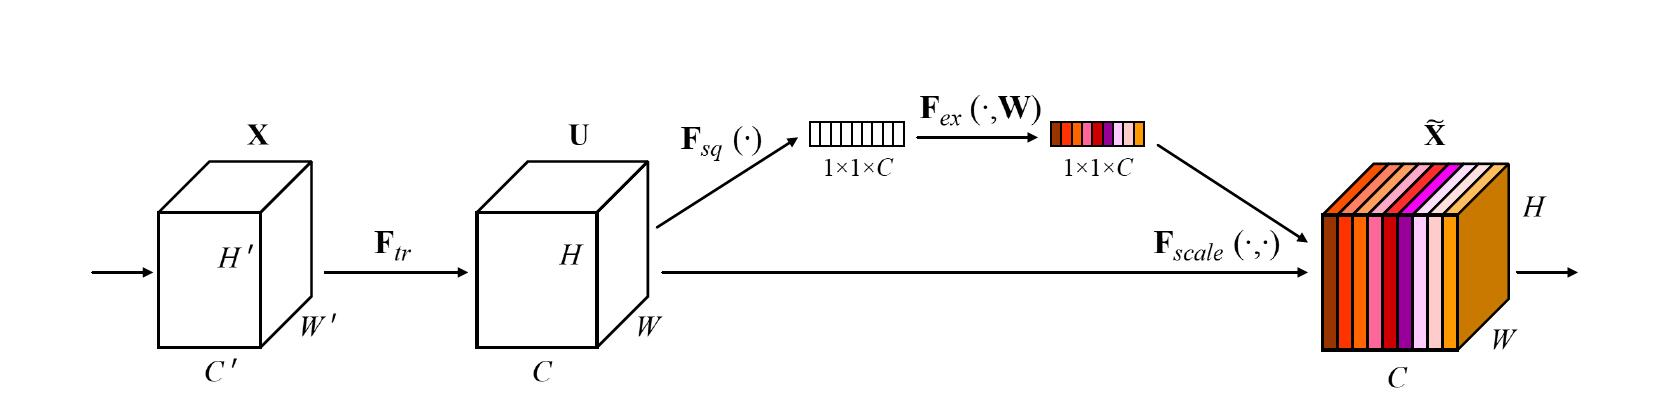
\includegraphics[width=14cm]{pic/chapter3/SENet.jpg}
    \caption{SENet 结构图\citing{hu2018squeeze}}
    \label{SENet}
\end{figure}

\subsection{空间注意力机制}
空间注意力机制是深度学习处理图像和空间数据中的注意力机制方法。其主要目的是通过对输入数据的不同空间位置引入不同的权重,赋予模型具备灵活关注对下游任务重要的区域的能力,提升模型对空间结构的感知能力。空间注意力模块(Spatial Attention Module, SAM)\citing{woo2018cbam}是一个经典的运用空间注意力机制的方法。如图\ref{SAM}所示,SAM的主要思想是首先利用最大池化层和平均池化层获得两个全局的特征图,然后通过拼接操作将两个特征图进行拼合,再利用一个$7\times 7$的卷积核将拼合的特征图转化成单通道的特征,最后使用sigmoid激活函数\citing{}得到空间注意力权值,并与原始输入进行相乘得到最终大小与输入相同的输出。空间注意力的计算公式如下式所示:
\begin{equation}
    \begin{aligned}
        \mathbf{M}_{\mathbf{s}}\left( \mathbf{F} \right) & =\sigma \left( f^{7\times 7}\left( \left[ AvgPool\left( \mathbf{F} \right) ;MaxPool\left( \mathbf{F} \right) \right] \right) \right)
        \\
                                                         & =\sigma \left( f^{7\times 7}\left( \mathbf{F}_{\mathbf{avg}}^{\mathbf{s}};\mathbf{F}_{\mathbf{max}}^{\mathbf{s}} \right) \right)
    \end{aligned}
\end{equation}

\begin{figure}[h]
    \centering
    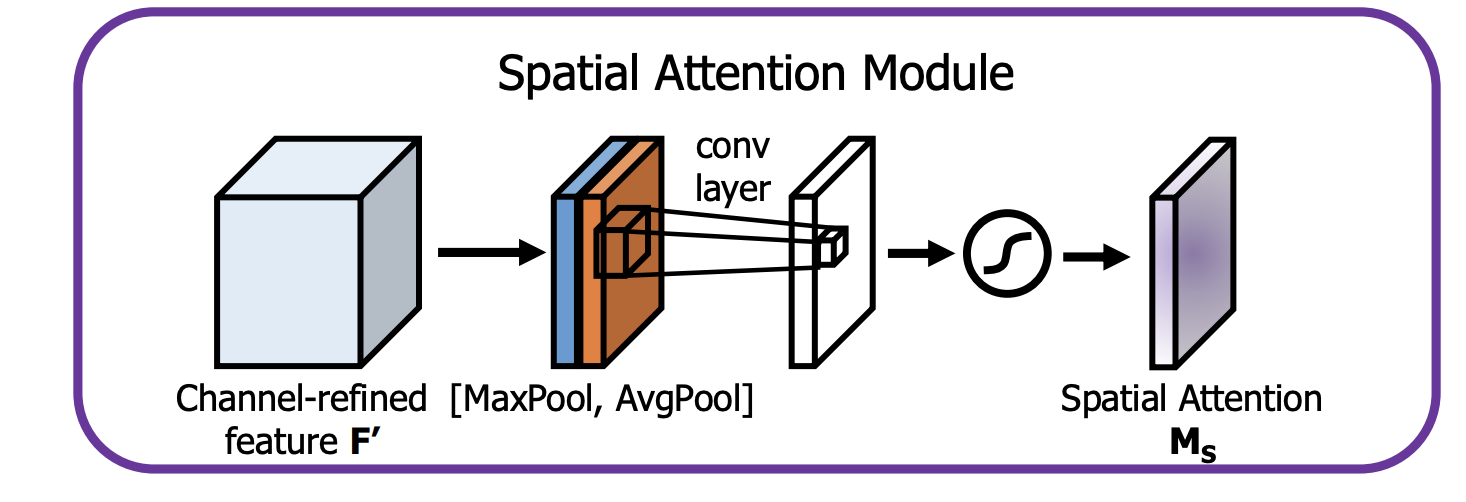
\includegraphics[width=14cm]{pic/chapter3/SAM.png}
    \caption{SAM 结构图\citing{woo2018cbam}}
    \label{SAM}
\end{figure}
\subsection{混合注意力机制}
混合注意力机制是综合多个注意力模块来处理数据的方法,通过对多个不同类型的注意力机制的融合,来增强深度网络模型对输入数据的建模能力,以更加灵活、全面地捕获输入数据的关键信息。卷积块注意力模块(Convolutional Block Attention Module, CBAM)\citing{woo2018cbam}是一个综合了通道和空间注意力机制的经典混合注意力方法。如图\ref{CBAM}所示,CBAM的主要网络架构有串联的通道注意力模块和空间注意力模块构成。通过依次使用通道和空间注意力模块,分别在通道和空间维度学习数据的关键信息,增强模型对输入数据的感知能力。其中,上一小节已经介绍了空间注意力模块的计算流程,而通道注意力机制的计算公式可以表示如下:
\begin{equation}
    \begin{aligned}
        \mathbf{M}_c\left( \mathbf{F} \right) & =\sigma \left( MLP\left( AvgPool\left( \mathbf{F} \right) \right) +MLP\left( MaxPool\left( \mathbf{F} \right) \right) \right)
        \\
                                              & =\sigma \left( \mathbf{W}_1\left( \mathbf{W}_0\left( \mathbf{F}_{avg}^{c} \right) \right) +\mathbf{W}_1\left( \mathbf{W}_0\left( \mathbf{F}_{max}^{c} \right) \right) \right)
    \end{aligned}
\end{equation}
其中,$\sigma$表示sigmoid函数,$W_0 \in \mathbb{R}^{C/r\times C}$、$W_1 \in \mathbb{R}^{C\times C/r}$均是多层感知机的权重参数。

因此,CBAM的计算流程可以表示为:
\begin{align}
    \mathbf{F}\prime=\mathbf{M}_{\mathbf{c}}\left( \mathbf{F} \right) \otimes \mathbf{F}
    \\
    \mathbf{F}''=\mathbf{M}_{\mathbf{S}}\left( \mathbf{F}\prime \right) \otimes \mathbf{F}\prime
\end{align}
其中,$\otimes$表示逐元素乘法。

\begin{figure}[h]
    \centering
    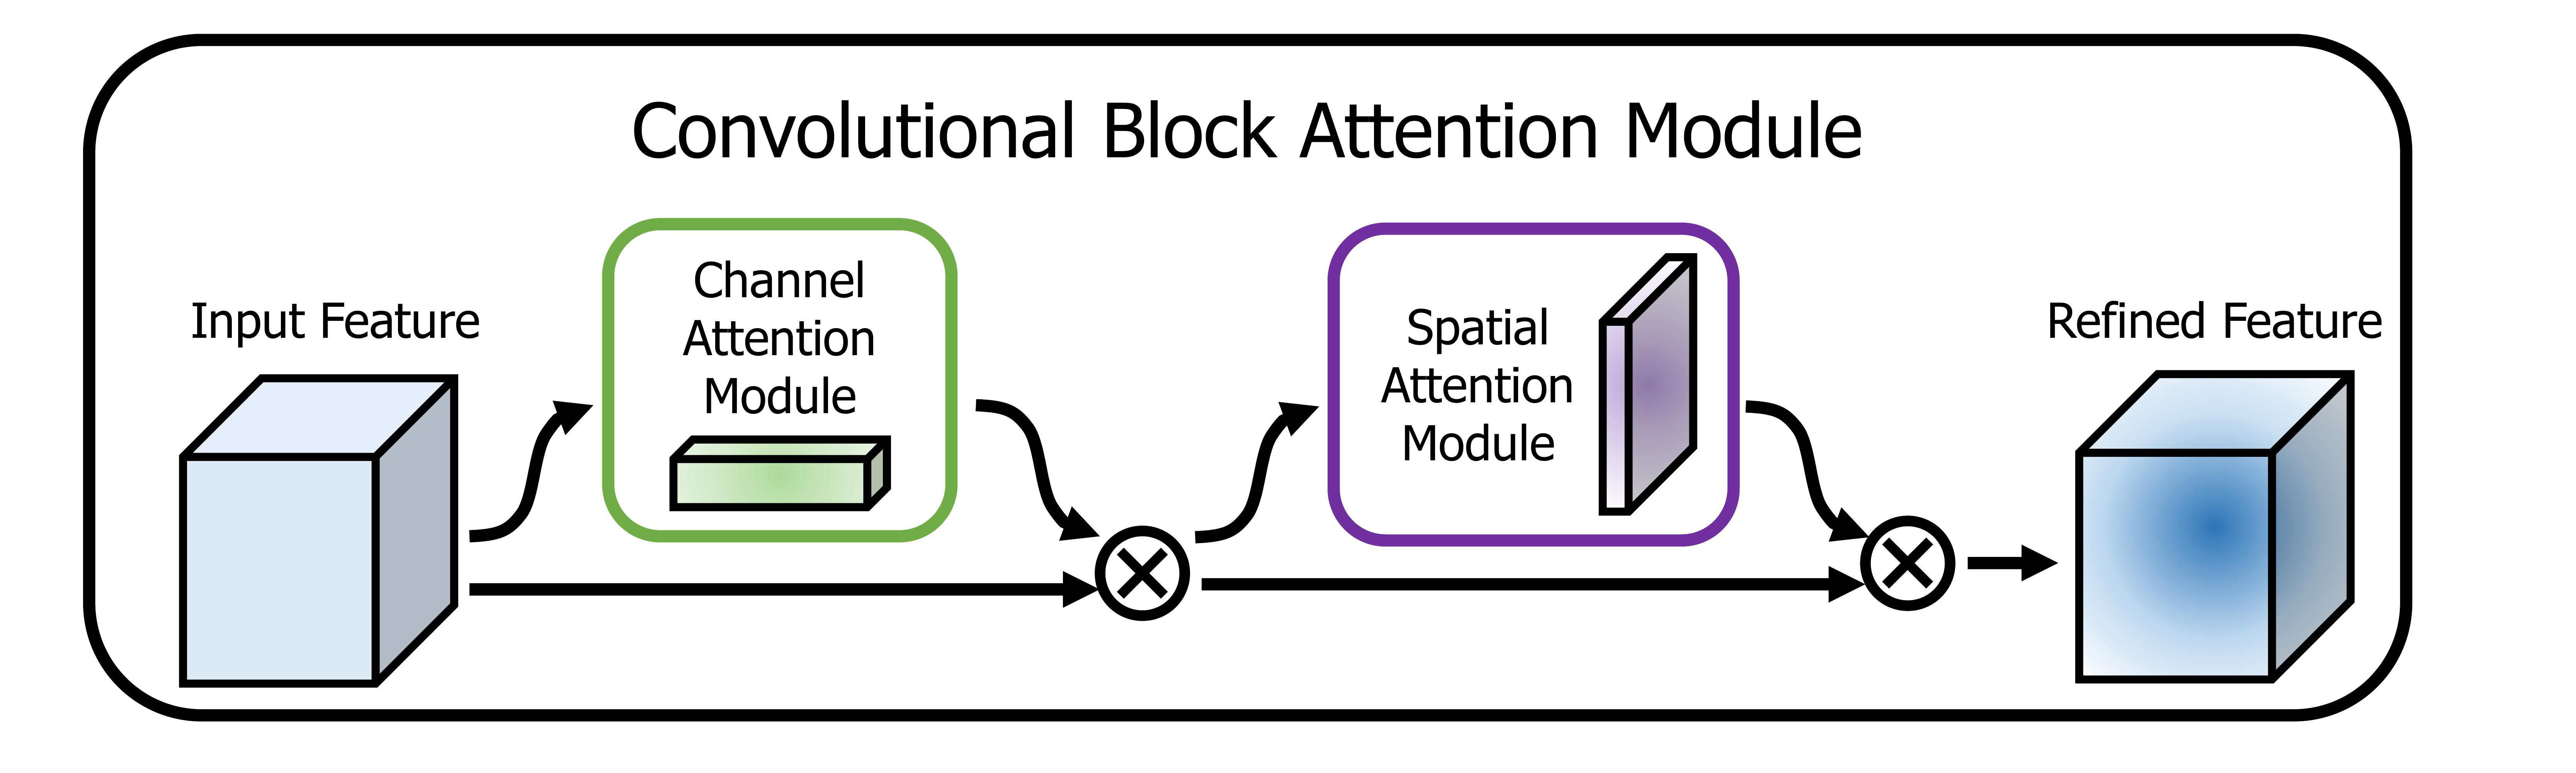
\includegraphics[width=14cm]{pic/chapter3/CBAM.jpg}
    \caption{CBAM 结构图\citing{woo2018cbam}}
    \label{CBAM}
\end{figure}

\section{基于双通道注意力的极化信息提取方法}
考虑到极化SAR图像原始数据可以由极化散射特征和极化目标分解特征进行表征,存在数据量大、信息复杂度高的问题,如果直接简单堆叠使用,甚至会导致模型性能下降。鉴于不同的地物目标之间散射特性存在差异,因此对极化SAR特征的重新标定校准是必不可少的,根据目标散射特性,自适应地增强有效特征,而抑制无效特征。为了高效地提取极化SAR数据中的有效信息,本章提出了一种基于双通道注意力的极化信息提取方法,旨在通过注意力机制来捕捉原始特征中的关键信息,充分考虑了不同极化特征之间的差异与联系,注重不同极化通道或空间中的关联性和权重分布,从而提高信息表征的准确性和效率。该方法可以作为一种即插即用的插件式网络结构,应用在后续的目标检测、地物分类任务中,为其提供更为可靠的基础极化信息表示。下面将详细介绍基于双通道注意力的极化信息提取方法的设计原理和实现步骤。

\subsection{双通道极化信息提取网络框架}
% 图\ref{DPEN_framework}是基于双通道注意力的极化信息提取算法示意图。该极化信息提取模型由两个注意力通道构成:极化目标分解通道和极化散射特征通道。该方法的主要思路是:首先通过设计双注意力通道的结构,将目标分解特征和散射特征隔离输入,保证模型对不同层次的特征具有感知能力。然后,在每一个通道内,依次采用空间注意力和通道注意力来捕获输入特征的关键信息。为了强化极化信息的感知能力,设计了极化注意力调整模块,聚合不同层次的关键信息,对得到的注意力权重进行修正。其次,为了进一步提升模型的空间信息学习能力,引入跨空间学习模块,聚合不同尺寸的极化特征。最后,将两个通道的极化信息拼接形成最终的注意力增强的极化特征,用于下游分类任务的输入。

图\ref{DPEN_framework}是基于双通道注意力的极化信息提取算法示意图。该极化信息提取方法主要目的是充分考虑散射特征和目标分解特征的关联性,通过设计合理网络结构来对两类信息的有效提取和整合。该算法框架的主要思路是:首先,通过双通道的结构形式,分别处理极化散射特征和目标分解特征,以实现对不同信息的有针对性提取,避免相互之间的干扰。其中一个通道专注于提取散射特征中的有效信息,而另一个通道专门处理目标分解特征。其次,在每个通道内部,采用通道注意力和空间注意力模块,以捕捉关键信息并增强空间、通道关键位置的权重,从而优化极化信息提取的准确性和处理效率。然后,设计了极化注意力调整模块,旨在通过极化散射的一致性修正两个通道之间的注意力权重,增强两者之间的协同作用。同时,为了对空间特征信息的建模,每个通道内部设置两个不同尺寸的分支,通过跨空间学习模块来保证模型对极化信息的全面感知能力。最后,通过拼接操作对两个通道中重新标定的特征进行融合输出,得到最终的有效极化信息表示,为后续任务提供可靠的数据基础。

\begin{figure}[h]
    \centering
    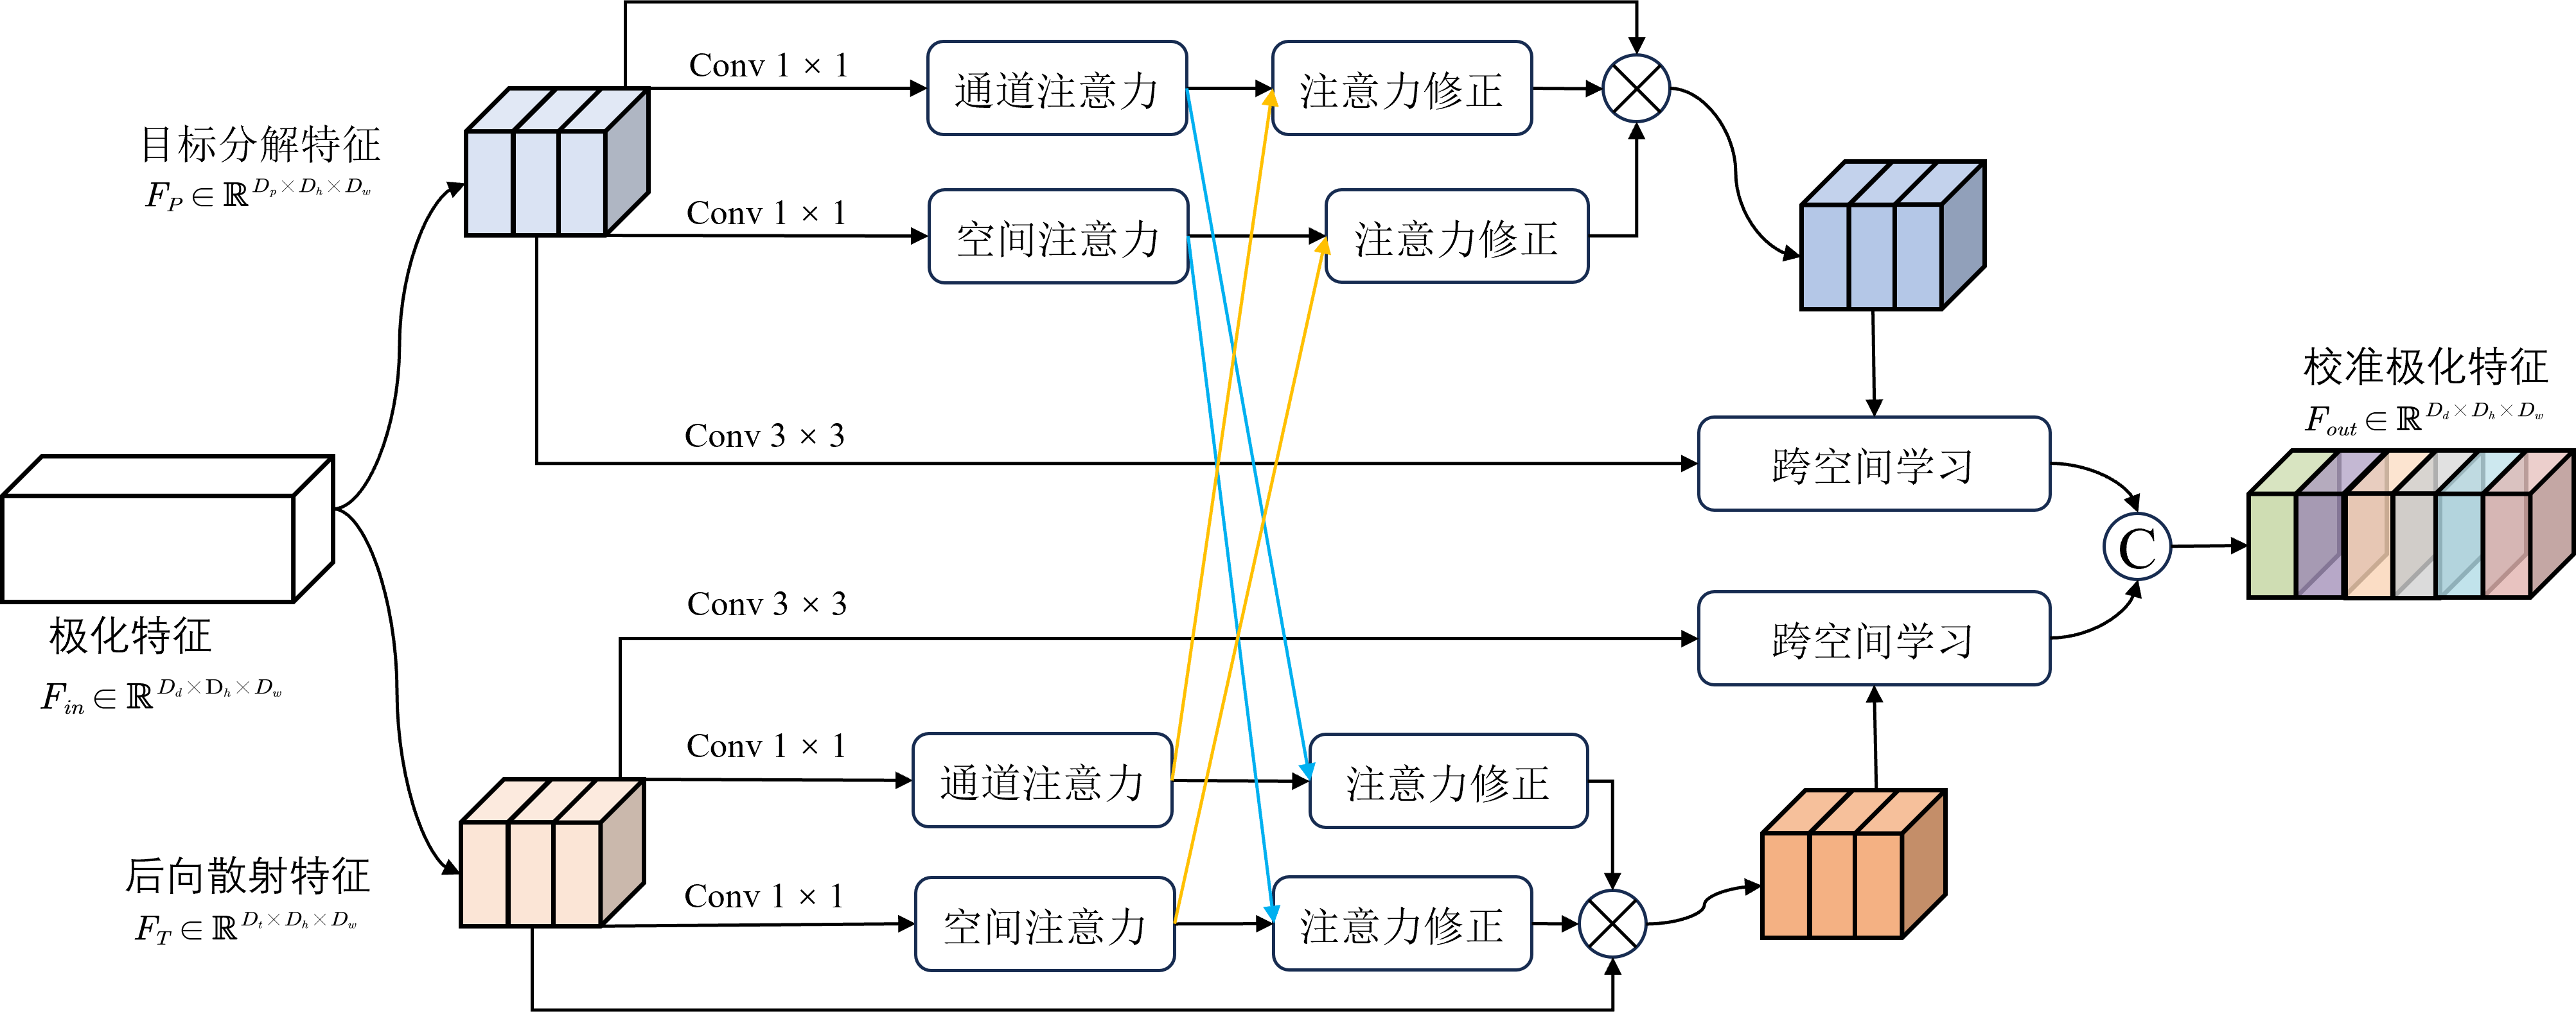
\includegraphics[width=14cm]{pic/chapter3/DPEN_framework.png}
    \caption{基于双通道注意力的极化信息提取算法示意图}
    \label{DPEN_framework}
\end{figure}


综合上述算法框架,基于双通道注意力的极化信息提取方法的主要步骤可以表示为以下几个步骤:

(1)极化原始特征提取。极化原始特征包含极化散射特征和极化目标分解特征两种不同层次的特征。利用不同的极化分解方法从极化SAR原始数据中提取出目标分解特征目标分解特征$x_D \in \mathbb{R}^{h\times w \times c_D}$。极化目标分解特征参数具体如表\ref{decomposision feature}所示。
\begin{table}[h]
    \caption{选用的极化目标分解特征}
    \begin{tabular}{cc}
        \hline \hline
        目标分解特征 & 描述             \\ \hline
        $\left| a \right|^2,\left| b \right|^2,\left| c \right|^2$
               & Pauli分解        \\ \hline
        $H,A,\alpha$
               & $H/A/\alpha$分解 \\ \hline
        $P_{hs},P_{hd},P_{hv}$
               & Freeman分解      \\ \hline \hline
    \end{tabular}
    \label{decomposision feature}
\end{table}

散射特征$x_S \in \mathbb{R}^{h\times w \times c_S}$,由极化相干矩阵中的元素构成,具体表示为:
\begin{equation}
    \begin{aligned}
        % TODO:
        F_S=\{T_{11},T_{22},real(T_{33}),real(T_{12}),real(T_{13}),
        \\
        image(T_{23}),image(T_{33}),image(T_{12}),image(T_{13}),image(T_{23})\}
    \end{aligned}
\end{equation}
其中,$real(\cdot)$表示取实数部分,$image(\cdot)$表示取虚数部分。

(2)极化关键信息提取。在两个通道中,利用通道注意力模块和空间注意力模块,提取关键的极化信息。通道注意力模块用于提取各通道内部的显著特征,而空间注意力模块用于增强空间位置重要的数据。通过为不同的通道与空间分配不同的权重,调整不同权重值的大小来改变对应空间与通道的特征在特征向量中的比值,增强不同散射体之间的联系。对于输入的极化特征$x_i \in \mathbb{R}^{h \times w \times c}$,空间和通道注意力模块输出不同空间通道的重要程度,如下式所示:
\begin{align}
    s_i=Attention_s\left( x_i \right)
    \\
    c_i=Attention_i\left( x_i \right)
\end{align}
其中,$Attention_s$和$Attention_c$分别表示空间和通道注意力计算函数,$i \in {1,2}$表示散射特征或目标分解特征。

(3)极化特征引导的注意力修正。

(4)跨空间特征学习。

(5)极化信息聚合。

最后将上述双通道注意力极化信息提取算法伪代码总结为表\ref{}。

\begin{algorithm}[H]
    \KwData{this text}
    \KwResult{how to write algorithm with \LaTeX2e}
    initialization\;
    \While{not at end of this document}{
        read current\;
        \eIf{understand}{
            go to next section\;
            current section becomes this one\;
        }{
            go back to the beginning of current section\;
        }
    }
    \caption{双通道注意力极化信息提取算法}
\end{algorithm}


\subsection{空间和通道注意力模块}
图\ref{}展示了本方法使用的注意力提取模块详细结构。

\subsection{极化注意力调整模块}
图\ref{DPEN_WFM}展示了极化注意力调整模块详细结构。
\begin{figure}[h]
    \centering
    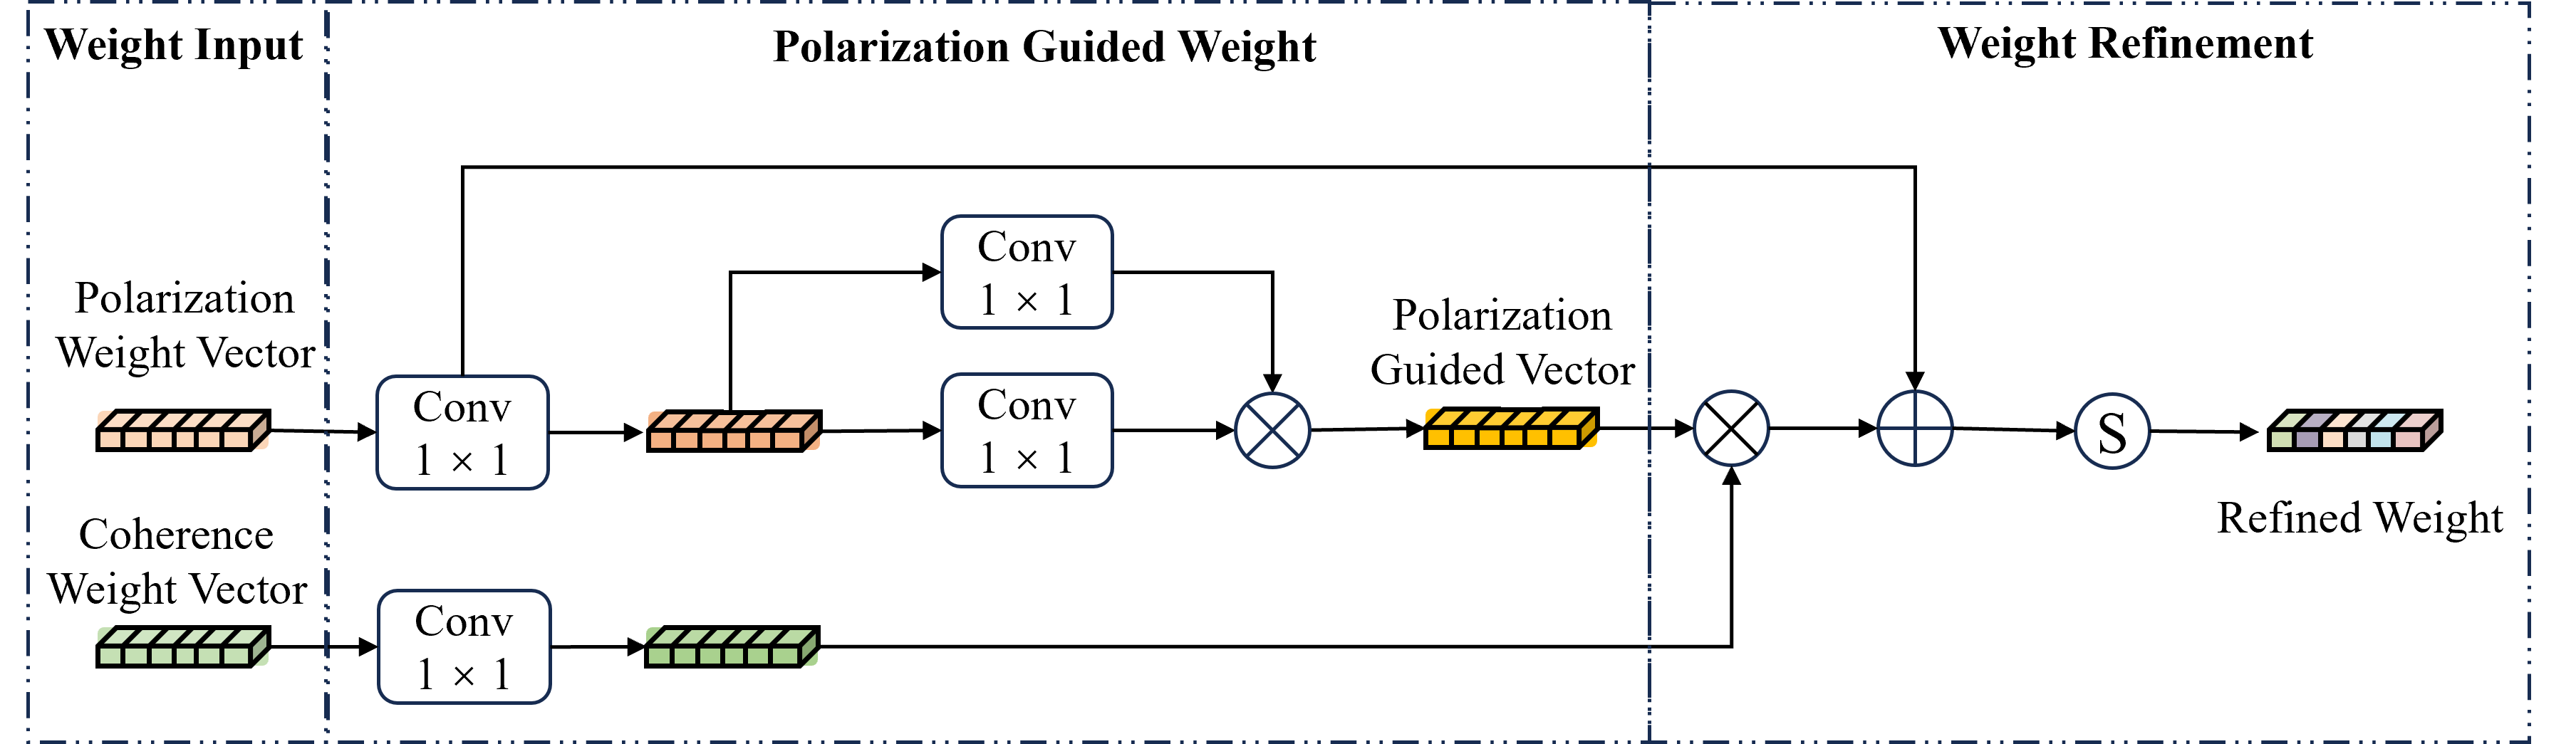
\includegraphics[width=14cm]{pic/chapter3/DPEN_WFM.png}
    \caption{极化注意力调整模块}
    \label{DPEN_WFM}
\end{figure}

\subsection{跨空间学习模块}
跨空间学习模块的网络结构如图\ref{DPEN_CSL}所示。
\begin{figure}[h]
    \centering
    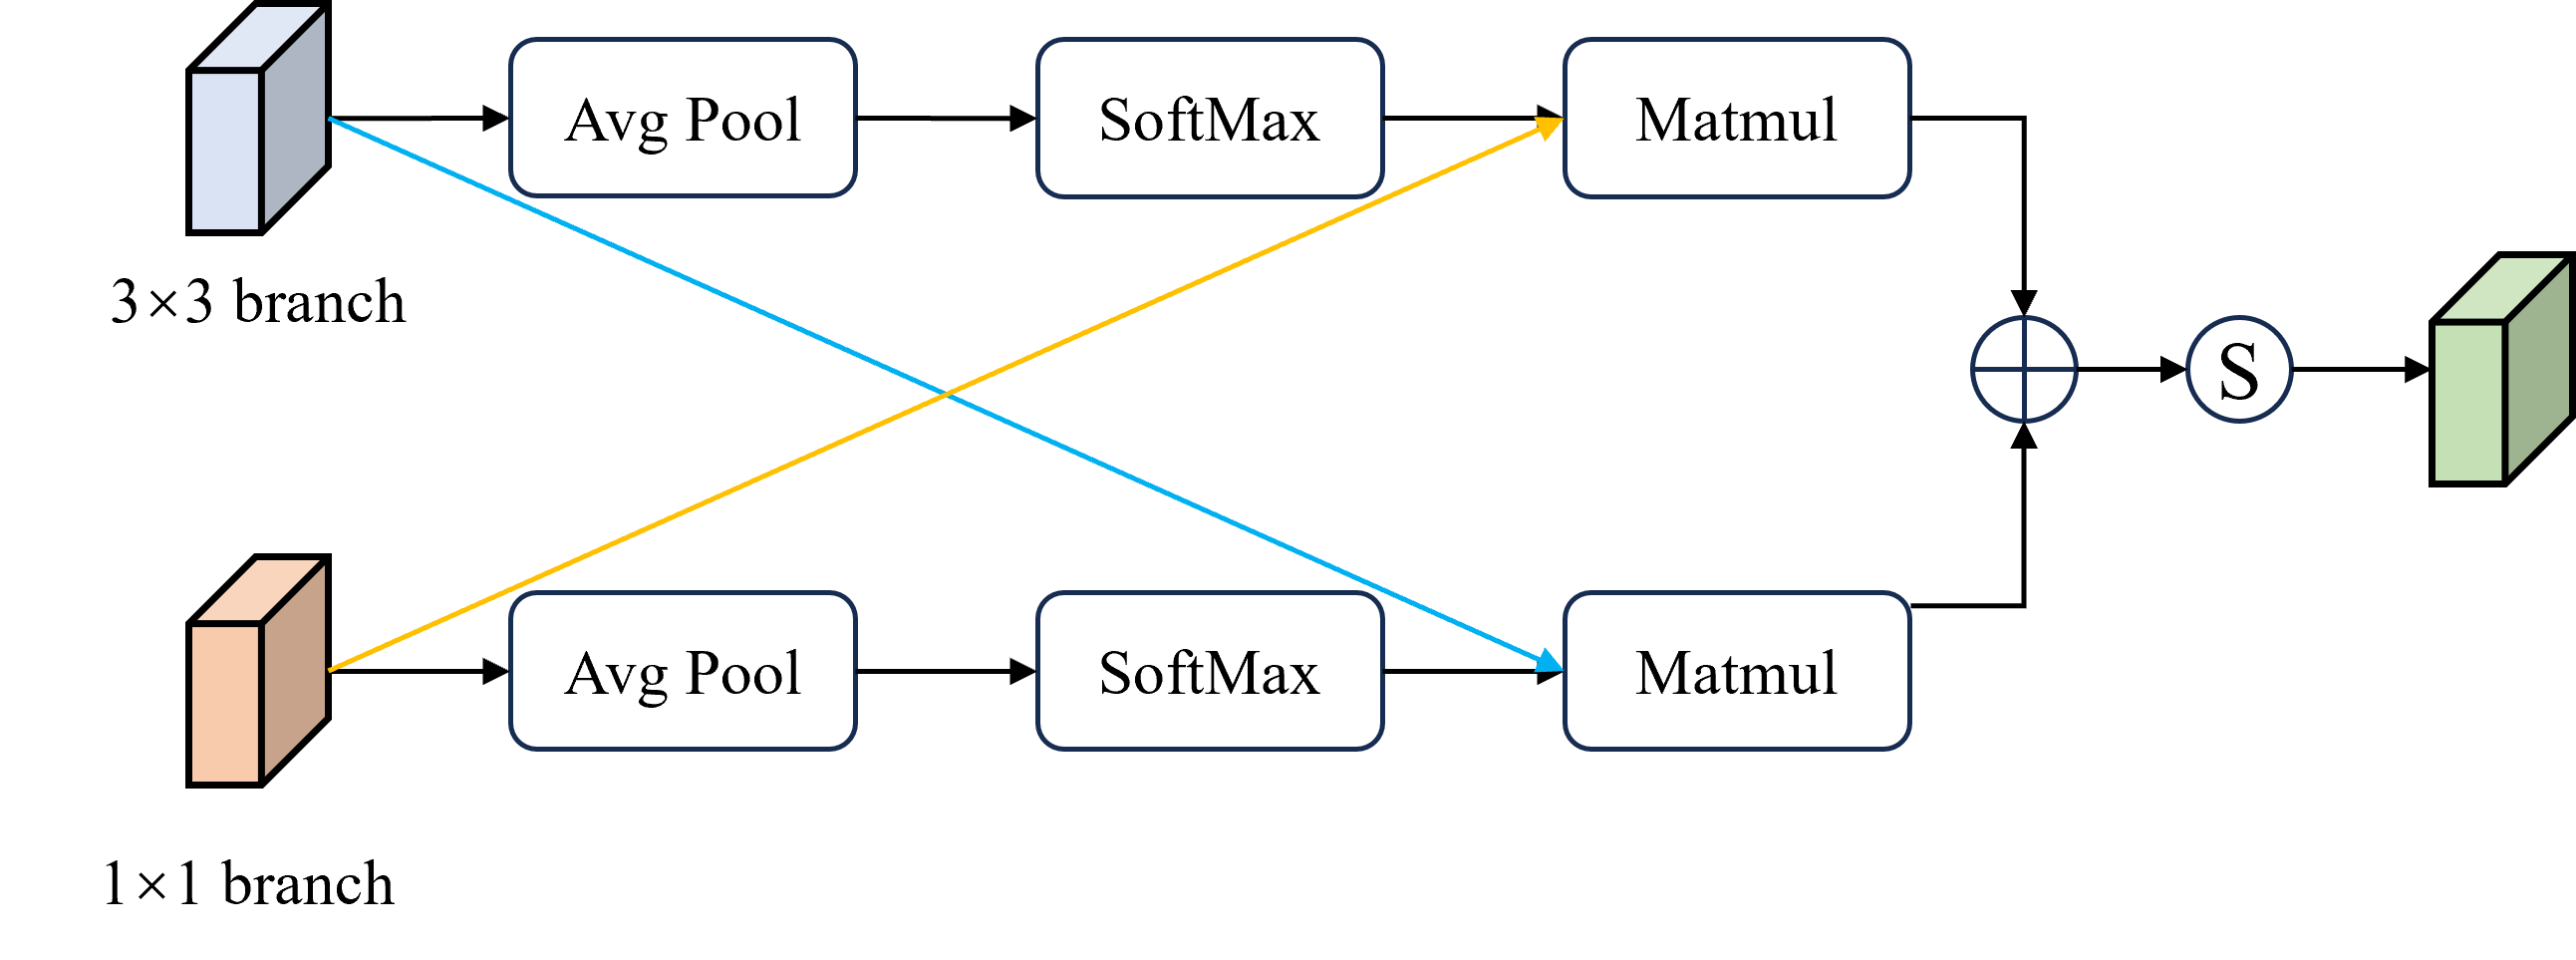
\includegraphics[width=14cm]{pic/chapter3/DPEN_CSL.png}
    \caption{CSL 结构图}
    \label{DPEN_CSL}
\end{figure}

\section{实验结果与分析}
为了验证本章方法的有效性,本节对本章提出的方法在多个极化SAR数据集上进行验证实验。采用多个常规的性能评价指标作为实验的数值量化标准:总体分类准确率(OA)、各个类别分类准确率(AA)和kappa系数。
\subsection{实验模型介绍}
本章实验在双通道注意力极化信息(Dual-Attention Polarization Information Extraction, DAPIE)提取方法基础上,构建端到端的极化特征提取与分类方法,记为DAPIE-CNN。DAPIE-CNN的结构如图\ref{}所示,分为极化信息提取和分类器两个部分。DAPIE模块作为模型的极化信息提取方法,用于对输入的高维极化特征进行有价值信息的激发和无价值信息的抑制。分类模块是对提取的极化信息进行精确的分类。

输入的极化特征如表\ref{pol-features}所示。
\begin{table}[ht]
    \caption{使用的极化特征列表}
    \resizebox{\linewidth}{!}{
        \begin{tabular}{ccc}
            \hline \hline
            极化特征         & 特征参数                                                & 特征数量 \\
            \hline
            Huynen       & T11,T22,T33                                         & 3    \\
            Freeman      & Freeman2(Vol,Ground),Freeman3(Odd,Dbl,Vol)          & 5    \\
            Cloude       & T11,T22,T33                                         & 3    \\
            H/A/$\alpha$ & alpha,anisotropy,beta,delta,entropy,gamma           & 6    \\
            Yamaguchi    & Yamaguchi3(Odd,Dbl,Vol),Yamaguchi4(Odd,Dbl,Vol,Hlx) & 7    \\
            Vanzyl       & Odd,Dbl,Vol,Hlx,Dbl-Hlx,wire                        & 6    \\
            \hline \hline
        \end{tabular}
    }
    \label{pol-features}
\end{table}

从输入的高维原始极化特征出发,利用DAPIE模块可以获得全局信息并且嵌入到分类器中。因此原始极化特征中有价值的信息被激发,而没有价值的信息被抑制。当具备了重新校正的极化特征之后,设计基于卷积神经网络(Convolution Neural Network, CNN)实现极化SAR图像的分类。在本节的实验验证方法中,遵循基于CNN的极化SAR分类的一般范式,使用一个类似vgg的卷积架构来拟合模型的特征输入。VggNet通过$3 \times 3$大小的堆叠卷积对经典的CNN进行改进,以获得更好的性能。分类模块的具体网络结构如表\ref{CNN-Vgg}所示。
\begin{table}[ht]
    \caption{分类模块网络结构}
    \begin{tabular}{ccc}
    \end{tabular}
    \label{CNN-Vgg}
\end{table}

以交叉熵损失函数\citing{}为目标,通过反向传播算法训练模型参数。交叉熵损失时分类问题中最常用的损失函数之一,衡量了分类模型的预测值与真实标签之间的差异性,是一种用于优化分类模型的目标函数。

综上所述,本章的DAPIE-CNN方法将输入的原始极化特征$x$映射为预测概率$p\in \mathbb{R}^{C}$,其中,$C$表示类别的个数。$x$对应的中心像素预测标签可以通过选择概率最高的类别,即向量$p$的最大值索引来预测。其计算公式如下:
\begin{equation}
    H(p,q)=\sum_{i=1}^{n}p(x_i)log(q(x_i))
\end{equation}
其中,$p(x)$表示真实值分布概率,$q(x)$表示模型预测分布概率。交叉熵值的变化与模型的训练效果密切相关,优越的训练效果会让预测概率分布逐渐趋近于真实值概率分布,相应的交叉熵值会逐渐减少。Sigmoid和Softmax损失函数是两个被广泛应用的交叉熵损失函数。Sigmoid损失函数主要应用于多标签分类任务,其中分类目标可以同时拥有多个标签。这一损失函数模拟了模型对多个独立事件的概率预测,每个事件的概率值落在$[0,1]$区间内。Softmax损失函数被广泛应用在多类别分类任务重,其中每个样本仅能关联一个类别。Softmax函数将预测模型的原始输出转化为表示类别概率的分布,确保所有类别的概率之和为1,并且模型的输出是互斥的。本章的极化SAR图像目标分类任务属于多分类语义分割任务,每个像素都有唯一的正确类别。因此选择多分类交叉熵损失函数,即Softmax损失函数作为模型的损失函数,这个选择侄子有效的应对单一正确标签的分类问题,并为模型训练提供有力的优化目标。


\subsection{精度评价方法}
精度评价是对实际数据和模型分类结果进行比较的重要步骤,旨在确定分类模型的准确性,是衡量分类结果可靠性的关键指标。混淆矩阵(Confusion Matrix)通常作为遥感图像分类准确性能的评判指标,并且可以通过混淆矩阵计算得到多种常用的评价参数指标,例如总体分类准确率(Overall Accuracy, OA)、各个类别分类准确率、各个类别平均分类准确率(Average Accuracy, AA)、Kappa系数等。

混淆矩阵是一个$n \times n$的矩阵,其中$n$表示数据集的类别数量。混淆矩阵的行表示实际类别,列表示预测类别。其中,每个元素$(i, j)$表示实际属于类别$i$的样本被预测为类别$j$的数量。混淆矩阵主对角线元素表示被正确分类的样本,非主对角线表示分类错误的样本。

在极化SAR图像分类结果精度评价中,可以基于混淆矩阵定义以下指标:

1.总体分类准确率(OA):
\begin{equation}
    OA=\frac{\mbox{主对角线元素之和}}{\mbox{混淆矩阵所有元素之和}}
\end{equation}

2.生产者精度:
\begin{equation}
    \mbox{生产者精度}=\frac{\mbox{类别对应的主对角线元素}}{\mbox{类别所在列总和}}
\end{equation}

3.使用者精度。
\begin{equation}
    \mbox{使用者精度}=\frac{\mbox{类别对应的主对角线元素}}{\mbox{类别所在行总和}}
\end{equation}

4.错分误差。
错分误差是指被分类模型错误地划分为用户感兴趣的类别,实际上属于另一类别的样本数量,反映了模型在预测时产生的误报情况。
\begin{equation}
    \mbox{错分误差}=1-\mbox{使用者精度}
\end{equation}

5.漏分误差。
漏分误差是指本应该属于地表真实分类的样本,但是由于模型未能正确分类而被判为其他类别的数量,反映了模型在预测时产生的漏报情况。
\begin{equation}
    \mbox{漏分误差}=1-\mbox{生产者精度}
\end{equation}

6.Kappa系数
Kappa系数是一种通过多元统计方法来评价分类精度的指标,旨在量化分类模型的性能相对于完全随机分类的优越性。该系数通过考察混淆矩阵的对角线元素以及总体分布情况,提供了对分类结果误差的全局度量。具体计算公式如下:
\begin{equation}
    K=\frac{p_0-p_e}{1-p_e}
\end{equation}
其中,$p_0$表示总体分类精度,由主对角线元素之和除以所有样本数量计算得到;$p_e$表示某一个类别地表真实样本总数与该类中被分类样本总数之积对所有类别求和除以总样本数的平方。将混淆矩阵中的具体元素带入上式,可以得到:
\begin{equation}
    K=\frac{N\sum_{i=1}^{r}{{x_i}_i}-\sum_{i=1}^{r}{\left( {x_i}_+x_{+i} \right)}}{N^2-\sum_{i=1}^{r}{\left( {x_i}_+x_{+i} \right)}}
\end{equation}

Kappa系数的大小可以用来表示分类的精度性能,表\ref{kappa}描述了Kappa系数与模型的分类精度的映射关系。
\begin{table}[ht]
    \caption{Kappa统计值与分类精度映射关系}
    \begin{tabular}{cc}
        \hline \hline
        Kappa系数 & 分类精度 \\
        \hline
        <0      & 较差   \\
        0-0.2   & 差    \\
        0.2-0.4 & 正常   \\
        0.4-0.6 & 好    \\
        0.6-0.8 & 较好   \\
        0.8-1   & 非常好  \\
        \hline \hline
    \end{tabular}
    \label{kappa}
\end{table}

\subsection{AIRSAR Flevoland数据实验}
实验数据集选择NASA/JPL于1989年在Flevoland区域采集得到的全极化数据。该数据集是荷兰的一个农业区域遥感数据,作为基准数据集广泛应用于极化SAR土地覆盖目标分类研究中。该图像大小为$1024 \times 750$ 像素,共有15种农作物类别,包括茎豆、豌豆、森林、苜蓿、小麦、甜菜、土豆、裸土、草、油菜籽、大麦、水和少量建筑物。各个农作物目标类别之间的差异较小,相似性较强,因此分类难度较大,容易出现错分漏分的现象。图\ref{flevoland_pauli}和图\ref{flevoland_gt}分别展示了AIRSAR Flevoland数据集的Pauli分解伪彩图像以及对应的地面真值标签图像。表\ref{flevoland_smaple}展示了该数据集中每个类别带标签的样本数量。
\begin{figure}[ht]
    \subfloat[]{
        \label{flevoland_pauli}
        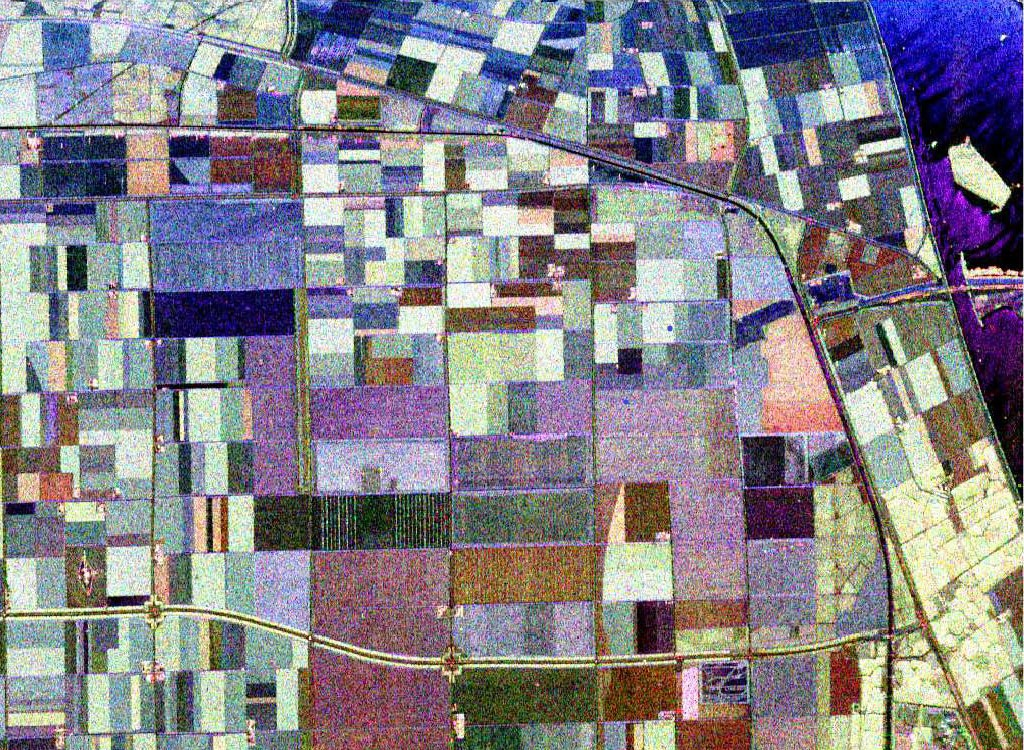
\includegraphics[width=7.04cm]{pic/chapter3/flevoland_pauli.png}
    }
    \subfloat[]{
        \label{flevoland_gt}
        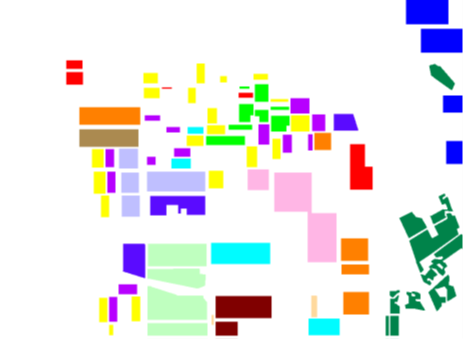
\includegraphics[width=7.04cm]{pic/chapter3/flevoland_gt.png}
    }
    \quad
    \subfloat[]{
        \label{pice}
        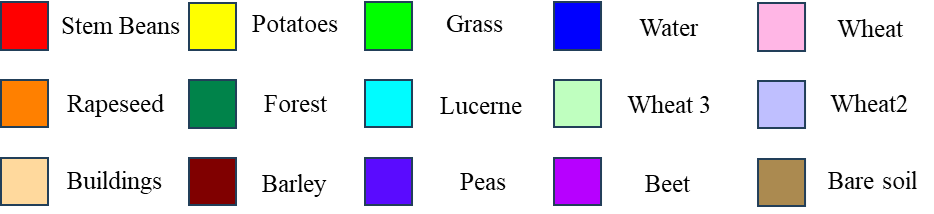
\includegraphics[width=9.04cm]{pic/chapter3/flevoland_label.png}
    }
    \caption{Flevoland地区实验数据集。(a)Pauli分解伪彩色图像;(b)实验数据地面真值;(c)颜色与类别对应关系}
    \label{fig2}
\end{figure}

\begin{table}[h]
    \caption{Felvoand地区实验数据集有标签样本数量}
    \resizebox{\linewidth}{!}{
        \begin{tabular}{|c|c|c|c|c|c|c|c|c|}
            \hline 类别 & steambeen & barley & bare soil & potato & beet     & wheat1 & peas  & lucerne \\
            \hline 数目 & 6338      & 7595   & 5109      & 16156  & 10033    & 11159  & 9582  & 10181   \\
            \hline 类别 & grass     & wheat2 & rapeseed  & wheat3 & building & forest & water &         \\
            \hline 数目 & 7058      & 16386  & 13863     & 22241  & 735      & 18044  & 13232 &         \\
            \hline
        \end{tabular}
    }
    \label{flevoland_smaple}
\end{table}


为了对本章提出的极化信息提取方法进行全面地评估和对比,选择了多种替代方案进行比较,主要涉及两个方面的变化:一方面是对特征输入的处理改变,另一方面是对极化信息提取模块的替代策略。首先在特征输入方面,探索了不同极化特征表示对目标分类任务的影响,包括输入极化特征为相干矩阵T的卷积网络(CNN-T)、输入为极化目标分解特征的卷积网络(CNN-P)、输入为全极化特征的卷积网络(CNN-F)以及以极化特征驱动的卷积网络(SF-CNN)\citing{}。其次,为了验证极化信息提取模块的有效性,尝试不同极化信息注意力调整模块和不同的结构进行对比,包括压缩和激励网络(SE-CNN)和空间通道注意力(CBAM)两种方法。

在每组实验中,从每个类别选择1\%的带标签像素,以这些带标签像素为中心,在其周围利用$15 \times 15$的窗口截取图像,形成训练集的特征表示。将从可视化分类结果、可视化特征分布以及精确量化结果来进行分析不同方法的性能。图\ref{}展示了不同方法的可视化分类结果。

\begin{figure}[ht]
    \subfloat[]{
        \includegraphics[width=4.04cm]{pic/pica.pdf}
    }
    \subfloat[]{
        \includegraphics[width=4.04cm]{pic/pica.pdf}
    }
    \subfloat[]{
        \includegraphics[width=4.04cm]{pic/pica.pdf}
    }
    \quad
    \subfloat[]{
        \includegraphics[width=4.04cm]{pic/pica.pdf}
    }
    \subfloat[]{
        \includegraphics[width=4.04cm]{pic/pica.pdf}
    }
    \subfloat[]{
        \includegraphics[width=4.04cm]{pic/pica.pdf}
    }
    \caption{AIRSAR Flevoland地区数据分类可视化结果图。(a)CNN-T;(b)CNN-P;(c)CNN-F;(d)SF-CNN;(e)CNN-T;(f)CNN-T}
    \label{fig2}
\end{figure}

可视化结果分析可视化结果分析可视化结果分析可视化结果分析可视化结果分析可视化结果分析可视化结果分析可视化结果分析可视化结果分析可视化结果分析可视化结果分析可视化结果分析可视化结果分析可视化结果分析可视化结果分析可视化结果分析可视化结果分析可视化结果分析可视化结果分析可视化结果分析可视化结果分析

为了进一步探索极化信息提取模块的性能,引入t-SNE(t-distributed Stochastic Neighbor Embedding)\citing{}特征分布图作为衡量极化信息提取模块的可视化评估指标。t-SNE是一种非线性降维技术,能够有效地将高维数据映射到二维或三维空间,以便更直观地观察样本在特征空间的分布。图\ref{}展示了不同数据特征通过t-SNE降维后的特征分布图。
\begin{figure}[ht]
    \subfloat[]{
        \includegraphics[width=4.04cm]{pic/pica.pdf}
    }
    \subfloat[]{
        \includegraphics[width=4.04cm]{pic/pica.pdf}
    }
    \subfloat[]{
        \includegraphics[width=4.04cm]{pic/pica.pdf}
    }
    \quad
    \subfloat[]{
        \includegraphics[width=4.04cm]{pic/pica.pdf}
    }
    \subfloat[]{
        \includegraphics[width=4.04cm]{pic/pica.pdf}
    }
    \subfloat[]{
        \includegraphics[width=4.04cm]{pic/pica.pdf}
    }
    \caption{AIRSAR Flevoland地区数据分类可视化结果图。(a)CNN-T;(b)CNN-T;(c)CNN-T;(d)CNN-T;(e)CNN-T;(f)CNN-T}
    \label{fle-tSNE}
\end{figure}

t-SNE结果分析t-SNE结果分析t-SNE结果分析t-SNE结果分析t-SNE结果分析t-SNE结果分析t-SNE结果分析t-SNE结果分析t-SNE结果分析t-SNE结果分析t-SNE结果分析t-SNE结果分析t-SNE结果分析t-SNE结果分析t-SNE结果分析t-SNE结果分析t-SNE结果分析t-SNE结果分析t-SNE结果分析t-SNE结果分析t-SNE结果分析t-SNE结果分析t-SNE结果分析t-SNE结果分析t-SNE结果分析t-SNE结果分析t-SNE结果分析t-SNE结果分析t-SNE结果分析t-SNE结果分析t-SNE结果分析t-SNE结果分析t-SNE结果分析t-SNE结果分析t-SNE结果分析t-SNE结果分析t-SNE结果分析t-SNE结果分析t-SNE结果分析t-SNE结果分析t-SNE结果分析t-SNE结果分析

采用总体准确率(OA)、平均准确率(AA)和Kappa系数三个指标对分类性能进行定量评价。精确分类量化评估结果如表\ref{fle_result}所示。
\begin{table}[ht!]
    % \renewcommand{\arraystretch}{1.5}
    % \setlength\tabcolsep{11pt}
    % \vspace{3cm} %调整图片与上文的垂直距离
    \centering
    \label{fle_result}
    \caption{AIRSAR Flevoland地区数据分类数值结果(\%)}
    \begin{tabular}{ccccccc}
        \hline\hline
        \text { Method }           & \text { SVM } & \text { SVM } & \text { SVM } & \text { Wishart } & \text { RSL } & \text { Ours } \\
        \hline \text { Buildings } & 37.26         & 37.26         & 37.26         & 32.64             & 35.34         & 96.38          \\
        \text { Rapeseed }         & 31.35         & 31.35         & 31.35         & 15.58             & 46.64         & 92.01          \\
        \text { Beet }             & 74.17         & 74.17         & 74.17         & 09.87             & 99.01         & 95.67          \\
        \text { Stembeans }        & 14.61         & 14.61         & 14.61         & 14.02             & 54.63         & 96.92          \\
        \text { Peas }             & 50.20         & 50.20         & 50.20         & 22.90             & 96.39         & 99.11          \\
        \text { Forest }           & 66.31         & 66.31         & 66.31         & 41.52             & 94.34         & 96.80          \\
        \text { Lucerne }          & 62.92         & 62.92         & 62.92         & 17.71             & 70.53         & 96.19          \\
        \text { Potatoes }         & 53.54         & 53.54         & 53.54         & 26.89             & 83.10         & 95.49          \\
        \text { Bare soil }        & 64.25         & 64.25         & 64.25         & 11.36             & 95.05         & 91.02          \\
        \text { Grass }            & 19.64         & 19.64         & 19.64         & 17.27             & 60.43         & 87.65          \\
        \text { Barley }           & 80.89         & 80.89         & 80.89         & 10.48             & 100.00        & 96.26          \\
        \text { Water }            & 76.90         & 76.90         & 76.90         & 59.90             & 59.32         & 97.37          \\
        \text { Wheat 1 }          & 59.13         & 59.13         & 59.13         & 40.18             & 91.83         & 97.71          \\
        \text { Wheat 2 }          & 45.27         & 45.27         & 45.27         & 46.52             & 70.16         & 94.82          \\
        \text { Wheat 3 }          & 75.74         & 75.74         & 75.74         & 43.69             & 98.85         & 97.05          \\
        \hline \text { OA }        & 58.98         & 58.98         & 58.98         & 49.78             & 89.13         & \textbf{95.85} \\
        \text { AA }               & 58.98         & 58.98         & 58.98         & 49.78             & 89.13         & \textbf{95.85} \\
        \text { Kappa }            & 56.02         & 56.02         & 56.02         & 47.16             & 89.12         & \textbf{95.47} \\
        \hline\hline
    \end{tabular}

\end{table}

数值结果分析数值结果分析数值结果分析数值结果分析数值结果分析数值结果分析数值结果分析数值结果分析数值结果分析数值结果分析数值结果分析数值结果分析数值结果分析数值结果分析数值结果分析数值结果分析数值结果分析数值结果分析数值结果分析数值结果分析数值结果分析数值结果分析数值结果分析数值结果分析数值结果分析数值结果分析数值结果分析数值结果分析

混淆矩阵混淆矩阵混淆矩阵混淆矩阵混淆矩阵混淆矩阵混淆矩阵混淆矩阵混淆矩阵混淆矩阵混淆矩阵混淆矩阵混淆矩阵混淆矩阵混淆矩阵混淆矩阵混淆矩阵混淆矩阵混淆矩阵混淆矩阵混淆矩阵混淆矩阵混淆矩阵混淆矩阵混淆矩阵混淆矩阵混淆矩阵混淆矩阵混淆矩阵混淆矩阵混淆矩阵混淆矩阵混淆矩阵混淆矩阵混淆矩阵混淆矩阵混淆矩阵混淆矩阵混淆矩阵混淆矩阵混淆矩阵混淆矩阵混淆矩阵混淆矩阵混淆矩阵混淆矩阵混淆矩阵

\subsection{AIRSAR San Francisco数据实验}
该数据集是由NASA/JPL的AIRSAR系统机载L波段的数据,测量了美国San Francisco Bay地区。该数据经过4视处理,具有高质量的全极化信息,是极化SAR目标分类研究的经典数据集之一。数据集大小为$1024\times 900$像素,入射角范围介于10°至60°之间。该数据集在方位向和距离向具有$10m \times 10m$的分辨率,利用Lee相干斑滤波器对其进行滤波处理。图\ref{san_pauli}和图\ref{san_gt}分别展示了该数据集的Pauli伪彩色图像和地面真值图像。

\begin{figure}[ht]
    \subfloat[]{
        \label{san_pauli}
        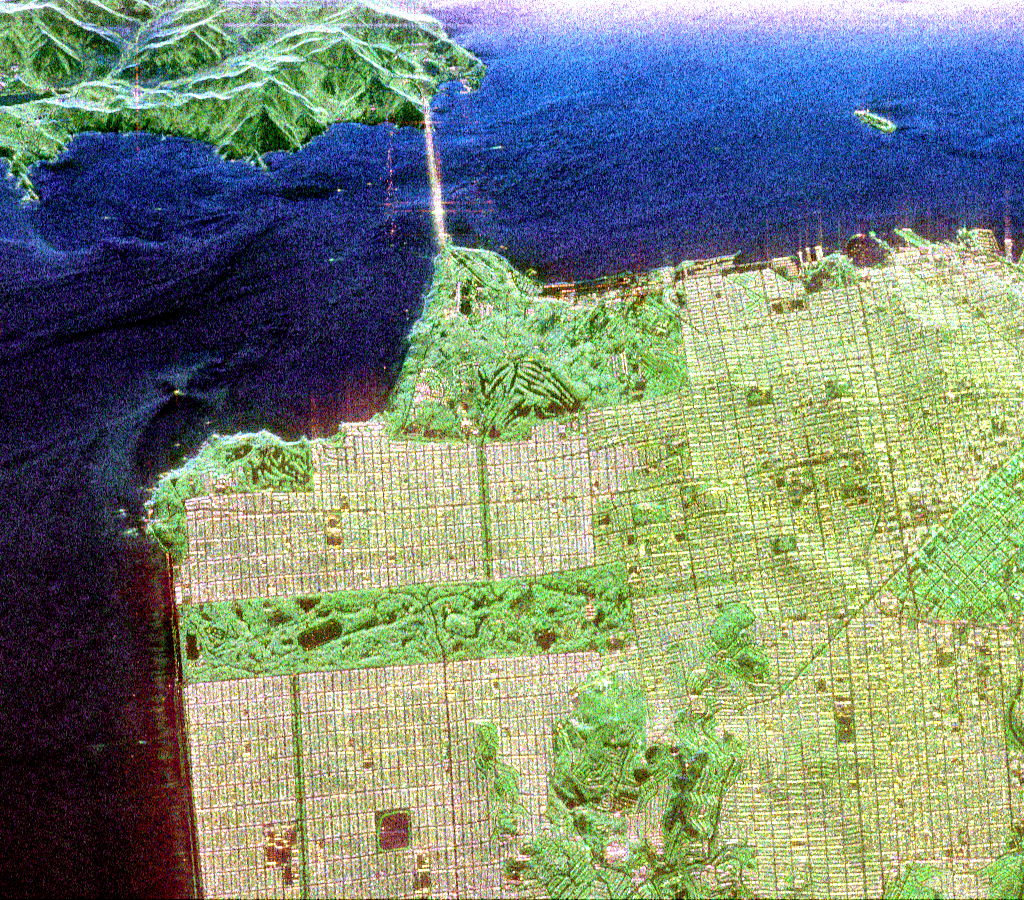
\includegraphics[width=7.04cm]{pic/chapter3/san_pauli.jpg}
    }
    \subfloat[]{
        \label{san_gt}
        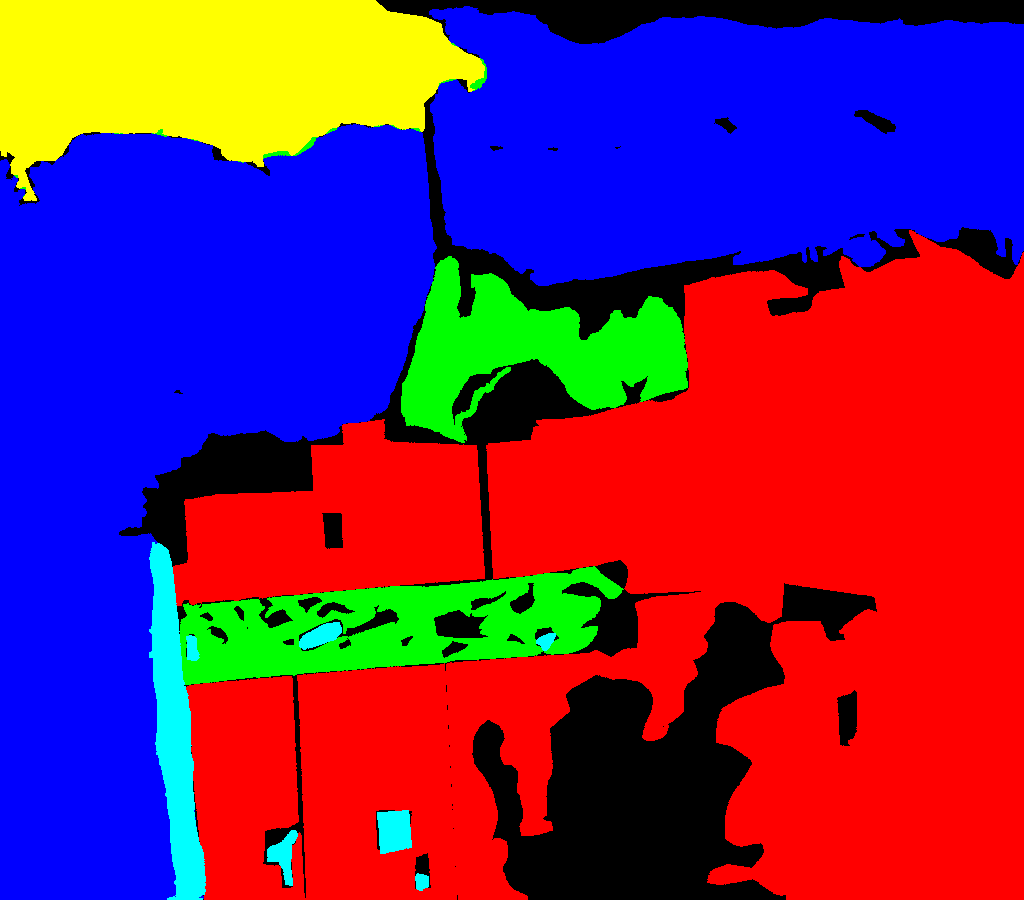
\includegraphics[width=7.04cm]{pic/chapter3/san_gt.png}
    }
    \quad
    \quad
    \subfloat[]{
        \label{pice}
        \includegraphics[width=9.04cm]{pic/chapter3/图片9.bmp}
    }
    \caption{San Francisco地区实验数据集。(a)Pauli分解伪彩色图像;(b)实验数据地面真值;(c)颜色与类别对应关系}
    \label{San}
\end{figure}

如图\ref{San}所示,该数据呈现了多样的地物目标景观,包含六种地面物体:建筑物、裸土、植被、山、水和其他地物。其中,图像的四周具有广阔的海洋区域,而左上角区域被茂密的植被覆盖,由金门大桥建筑区域与下方的地物连接。图像中部为公园区域,公园周围属于城市居民区域,而图像的右方则呈现出一个近似三角形的植被覆盖区域。这些不同的地物类型分布丰富多彩,为地物分类和遥感研究提供了丰富的实例和场景。

图像中每个类别带有标签的样本数量如表\ref{san_smaple}所示。

\begin{table}[h]
    \caption{San Francisco地区实验数据集有标签样本数量}
    \resizebox{\linewidth}{!}{
        \begin{tabular}{|c|c|c|c|c|c|c|c|c|}
            \hline 类别 & steambeen & barley & bare soil & potato & beet     & wheat1 & peas  & lucerne \\
            \hline 数目 & 6338      & 7595   & 5109      & 16156  & 10033    & 11159  & 9582  & 10181   \\
            \hline 类别 & grass     & wheat2 & rapeseed  & wheat3 & building & forest & water &         \\
            \hline 数目 & 7058      & 16386  & 13863     & 22241  & 735      & 18044  & 13232 &         \\
            \hline
        \end{tabular}
    }
    \label{san_smaple}
\end{table}

\section{本章小结}
本章针对极化ASR图像信息利用中所面临的信息冗余问题,提出了一种基于双通道注意力的极化信息提取方法。通过构建极化散射特征通道和目标分解特征通道的双通道结构,结合空间、通道注意力机制,能够有效地提取出两种不同类型的极化特征中的关键极化信息。为了增强两种信息的关联,设计了散射特征导向的注意力修正方法,对注意力权重进行修正,从而全面聚合关键极化信息。最后设计多尺度特征学习模块,赋能模型对不同尺度极化信息的捕捉能力。最后通过视觉和数据量化两个层面进行性能评估,结果表明本章提出的方法能够有效地提升极化数据中的信息表征方式,从而提升极化SAR图像的分类精度。